%group_pres.tex

\documentclass{beamer}
\mode<presentation>
\usetheme{default}

\usepackage{graphicx}                  %use package for diagram 
\usepackage{amsmath}                   %use package for implies symbol
\usepackage{amsfonts}		       %use package for numbet sets
\usepackage{bm}                        %use package for bolds in math mode
\usepackage{tikz}                      %use package for diagram drawings
\usepackage{algpseudocode}             %use package for pseudocode
\usepackage{algorithm}                 %use package for pseudocode
\usepackage[justification=centering]{caption}                   %use package for multiple figures
\usepackage{subcaption}                %use package for multiple figures
\usepackage{color}                     %use package for code listings
\usepackage{listings}                  %use package for c++ code in appendix
\usepackage[utf8]{inputenc}            %use package for colours in code
\usepackage{array}                     %use package for centering table contents
\usepackage{microtype}		       %use package for small typographical changes

%define colours for code listings
\definecolor{codegreen}{rgb}{0,0.6,0}
\definecolor{codegray}{rgb}{0.5,0.5,0.5}
\definecolor{codepurple}{rgb}{0.58,0,0.82}
\definecolor{backcolour}{rgb}{0.95,0.95,0.92}

%define a style for the listings
\lstdefinestyle{mystyle}{
    backgroundcolor=\color{backcolour},
    commentstyle=\color{codegreen},
    keywordstyle=\color{magenta},
    numberstyle=\tiny\color{codegray},
    stringstyle=\color{codepurple},
    basicstyle=\footnotesize,
    breakatwhitespace=false,
    breaklines=true,
    captionpos=b,
    keepspaces=true,
    numbers=left,
    numbersep=5pt,
    showspaces=false,
    showstringspaces=false,
    showtabs=false,
    tabsize=2,
    language=C++
}

%set style of listing to that defined above
\lstset{style=mystyle}

%set style of footnotes
\renewcommand{\thefootnote}{\roman{footnote}}

%define command shortcuts
\newcommand{\be}{\begin{equation}}
\newcommand{\ee}{\end{equation}}

%use tikz library for shapes
\usetikzlibrary{shapes.geometric, arrows}

%define block styles in tikz
\tikzstyle{startstop} = [rectangle, rounded corners, minimum width=3cm, minimum height=1cm, text centered, draw=black, fill=red!30]
\tikzstyle{io} = [trapezium, trapezium left angle=70, trapezium right angle=110, minimum width=3cm, minimum height=1cm, text centered, draw=black, fill=blue!30]
\tikzstyle{process} = [rectangle, minimum width=3cm, minimum height=1cm, text centered, draw=black, fill=orange!30]
\tikzstyle{decision} = [diamond, minimum width=3cm, minimum height=1cm, text centered, draw=black, fill=green!30]
\tikzstyle{arrow} = [thick,->,>=stealth]

%set graphics path
\graphicspath{{/home/danmfr/p3t/laplace/images/}}

\title{$3^{rd}$ Year Theoretical Physics Group Project}
\subtitle{On numerical solutions to Laplace's equation for different boundary conditions}
\author{S. Brown, F. Hayes, L. Heikkil{\"a}, D. Richardson\\
        School of Physics and Astronomy,\\
        University of Glasgow,\\
        Glasgow, United Kingdom}
\date{\today}

%layout page at start of new section
\AtBeginSection[]
{
  \begin{frame}<beamer>
    \frametitle{Layout}
    \tableofcontents[currentsection,currentsubsection]
  \end{frame}
}

\begin{document} %start of document

\begin{frame} 
\titlepage
\end{frame}

\begin{frame}
\tableofcontents
\end{frame}

\section{Overview}
\begin{frame}{Overview}
Aims:
\begin{itemize}
\item introduce and derive the Laplace equation and list its uses
 \begin{itemize}
 \item start with general solution, find a particular solution
 \end{itemize}
\item introduce finite difference methods and discuss their necessity
\item introduce and describe software package 
 \begin{itemize}
 \item present results and analysis of software package
 \end{itemize}
\end{itemize}

This discussion of the Laplace equation occurs within EM but can
be generalised to other physical phenomena where the equation occurs:
\begin{itemize}
\item thermodynamics,
\item fluid mechanics,
\item astronomy.
\end{itemize}
\end{frame}

\section{Introduction}
\subsection{Derivation of Laplace's Equation}

\begin{frame}{Derivation of Laplace's Equation in Electromagnetism}
Consider two of Maxwell's equations, Gauss' Law and Faraday's Law:
%
\be
\nabla \cdot \bm{E} = \frac{\rho}{\epsilon_0} \qquad \nabla \times \bm{E} = -\frac{\partial \bm{B}}{\partial t}
\ee

In static free space:
\begin{itemize}
 \item $\bm{B}$ is unchanging $\implies$ $\bm{E}$ is irrotational $\implies \bm{E} = -\nabla \phi$
 \item $\rho=0$ $\implies \bm{E}$ is solenoidal $\implies \nabla^2 \phi = 0$.
\end{itemize}

This is Laplace's equation.
\begin{itemize}
 \item $2^{nd}$ order PDE that can be solved to find $\phi$ and hence $\bm{E}$
 \item $\bm{E}$ allows equation of motion of test particles to be found (Lorentz force)
\end{itemize}
\end{frame}

\subsection{Physical Systems}

\begin{frame}{Electrostatic Systems}
\begin{figure}
\centering
\begin{subfigure}[b]{0.45\textwidth}
	\centerline{\includegraphics[scale=0.4, trim = 0cm 1cm 0cm 0cm, clip=true]{sysA.pdf}}
	\caption{System A}
\end{subfigure}
\hfill
\begin{subfigure}[b]{0.45\textwidth}
	\centerline{\includegraphics[scale=0.4, trim = 0cm 1cm 0cm 0cm, clip=true]{sysC.pdf}}
	\caption{System C}
\end{subfigure}
\caption{Cross-sectional diagram of two electrostatic systems}
\end{figure}

\end{frame}

\subsection{Analytical Solution of System A}

\begin{frame}{General Analytical Solution}
\begin{figure}
\centering
	\begin{tikzpicture}
	\draw (0,0) -- (0,2.5) node[above, font=\footnotesize] {$\phi = V$}; 
	\draw (4.2,0) -- (4.2,2.5) node[above, font=\footnotesize] {$\phi = -V$}; 
	\draw (2.1,1.25) circle (0.5cm) node[below, font=\footnotesize, yshift=-0.4cm] {GND};
	\draw[dashed] (2.1,1.25) -- (2.5,1.55) node[pos=0.2, above, font=\footnotesize,] {$R$};
	\end{tikzpicture}
	\caption{System A}
\end{figure}

Exploit the symmetry of the system by finding the general solution of $\nabla^2 \phi=0$
in plane polar co-ordinates: 
%
\be
\frac{1}{r}\frac{\partial}{\partial r}\left(r \frac{\partial \phi}{\partial r}\right) + \frac{1}{r^2}\frac{\partial ^2 \phi}{\partial \theta^2} = 0 
\ee

Separate variables, $\phi(r,\theta)=f(r)g(\theta)$. Substitution gives
%
\be
\frac{r}{f(r)}\frac{d}{dr}\left(r \frac{df(r)}{dr}\right) =- \frac{1}{g(\theta)}\frac{d^2 g(\theta)}{d \theta^2}
\ee

\end{frame}

\begin{frame}{General Analytical Solution cont.}
We had that:
%
\be
\frac{r}{f(r)}\frac{d}{dr}\left(r \frac{df(r)}{dr}\right) =- \frac{1}{g(\theta)}\frac{d^2 g(\theta)}{d \theta^2}
\ee
%
Left-hand side is solely a function of $r$; right-hand side of $\theta$ 
\begin{itemize}
\item both sides must be constant, $k^2$ say, for some $k \in \mathbb{R}$.
\end{itemize}

Produces pair of second-order ODEs:
%
\be
r\frac{d}{dr}\left(r \frac{df(r)}{dr}\right) = k^2 f(r) \quad \frac{d^2 g(\theta)}{d\theta^2} = -k^2 g(\theta)
\ee

\end{frame}

\begin{frame}{General Analytical Solution cont.}
Solutions of two ODEs:
\begin{itemize}
\item $k=0$:
\be
f(r)=\alpha_0 \ln(r) + \beta_0  \quad \text{and} \quad g(\theta)=\gamma_0 \theta +\delta_0
\ee
\item $k \neq 0$:
\be
f(r)=\alpha_k r^k +\beta_k r^{-k} \quad \text{and} \quad g(\theta) = \gamma_k \sin(k\theta) +\delta_k \cos(k\theta)
\ee
\end{itemize}

Expect $g$ to be single-valued: $g(\theta+2\pi)=g(\theta) \implies k \in \mathbb{Z}$.

Principle of superposition gives general solution of Laplace's equation in polar
co-ordinates:
%
\begin{multline}
\phi(r, \theta) = (\alpha_0 \ln(r) + \beta_0)(\gamma_0\theta + \delta_0) \\
                + \sum_{n=1}^{\infty}(\alpha_n r^n+\beta_n r^{-n})(\gamma_n \sin(n\theta) + \delta_n \cos(n\theta))
\end{multline}

\end{frame}

\begin{frame}{Particular Solution for System A}
To find particular solution we impose \emph{Dirichlet boundary conditions}.

We have the general solution
%
\begin{multline}
\phi(r, \theta) = (\alpha_0 \ln(r) + \beta_0)(\gamma_0\theta + \delta_0) \\
                + \sum_{n=1}^{\infty}(\alpha_n r^n+\beta_n r^{-n})(\gamma_n \sin(n\theta) + \delta_n \cos(n\theta))
\end{multline}

Conditions:
\begin{itemize}
\item $\phi$ is symmetric in $\pm\theta$ or about $\theta=0 \implies \gamma_n=0, \; \forall n$
\item $\phi$ is finite at infinity $\implies \alpha_n=0, \; \forall n$
\end{itemize}

Hence
%
\be
\phi(r, \theta) = \beta_0 + \sum_{n=1}^{\infty} \frac{\beta_n}{r^n} \cos(n\theta)
\ee
%
where the $\beta$'s absorbed other constants.
\end{frame}

\begin{frame}{Particular Solution for System A cont.}
We have
%
\be
\label{eq:sum}
\phi(r, \theta) = \beta_0 + \sum_{n=1}^{\infty} \frac{\beta_n}{r^n} \cos(n\theta)
\ee

As $r \rightarrow \infty$, $\phi$ is linearly decreasing between the plates:
%
\be
\phi \rightarrow -\frac{Vx}{d}=-\frac{Vr}{d}\cos(\theta)
\ee.

Thus, $\beta_0=-\frac{Vr}{d}\cos(\theta)$, since the $2^{nd}$ term in eq.~\ref{eq:sum} 
vanishes.

Then,
%
\be
\phi(r, \theta) = -\frac{Vr}{d}\cos(\theta) + \sum_{n=1}^{\infty} \frac{\beta_n}{r^n} \cos(n\theta)
\ee
%
or,
%
\be
\phi(r, \theta) = \left(\frac{\beta_1}{r}-\frac{Vr}{d}\right)\cos(\theta) + \sum_{n=2}^{\infty} \frac{\beta_n}{r^n} \cos(n\theta)
\ee

\end{frame}

\begin{frame}{Particular Solution for System A cont.}
We have
%
\be
\phi(r, \theta) = \left(\frac{\beta_1}{r}-\frac{Vr}{d}\right)\cos(\theta) + \sum_{n=2}^{\infty} \frac{\beta_n}{r^n} \cos(n\theta)
\ee

Expect continuity of $\phi$ at the surface of the cylinder:
%
\be
\phi(r=R,\theta) = 0 \implies \beta_1=\frac{VR^2}{d} \quad
\text{and} \quad \beta_{n \geq 2} = 0
\ee
%
since the set $\{\cos(n \theta)\}$ are linearly independent functions.

Final solution is:
%
\be
\phi(r, \theta) = \frac{V}{d}\left(\frac{R^2}{r}-r\right)\cos(\theta)
\ee
for $r>R$ and $0$ otherwise.

\end{frame}

\begin{frame}{Analytical Solution}

\begin{figure}[h!]
\begin{center}
\includegraphics[scale=0.8]{analytic.pdf}
\caption{Analytic solution with $V=1$, $R=15$, $d=50$}
\end{center}
\end{figure}

\end{frame}

\section{Numerical Methods}
\begin{frame}{Necessity of Numerical Methods}
Analytically solvable systems are few and far-between.

In general, it is difficult, and often impossible, to express systems mathematically
in terms of algebraically utilisable boundary conditions and impose these conditions
on general solutions of Laplace's equation in given co-ordinates.

Solutions to these types of systems must be numerically approximated.

One such way is Finite Difference Methods.
\end{frame}

\subsection{Finite Difference Methods}

\begin{frame}{Finite Difference Methods}
We use the definition of the derivative, for a function $f(t)$ say, and approximate as
%
\be
\frac{df}{dt} = \lim_{\Delta t\to 0}\frac{f(t+\Delta t) - f(t)}{\Delta t} \approx \frac{f(t+\Delta t) - f(t)}{\Delta t}
\ee
%
where $\Delta t$ is assumed to be small enough that the approximation is good.

We can then approximate the second derivative similarly:
%
\begin{align}
\frac{d^2 f}{dt^2} &\approx \frac{f'(t+\Delta t) - f'(t)}{\Delta t} \\
		   &= \frac{\frac{f(t+\Delta t) - f(t)}{\Delta t} - \frac{f(t) - f(t-\Delta t)}{\Delta t}}{\Delta t} \\
\frac{d^2 f}{dt^2} &\approx  \frac{f(t+\Delta t) - 2f(t) + f(t-\Delta t)}{\Delta t^2}
\end{align}

\end{frame}

\begin{frame}{Finite Difference Methods cont.}

Define a region on which to discretise Laplace equation, 
%
\be
\Omega = \{(x,y)|\:0<x<L,0<y<D\}
\ee

Create a grid of points in $\Omega$ at which to solve the equation:

\begin{figure}
\centering
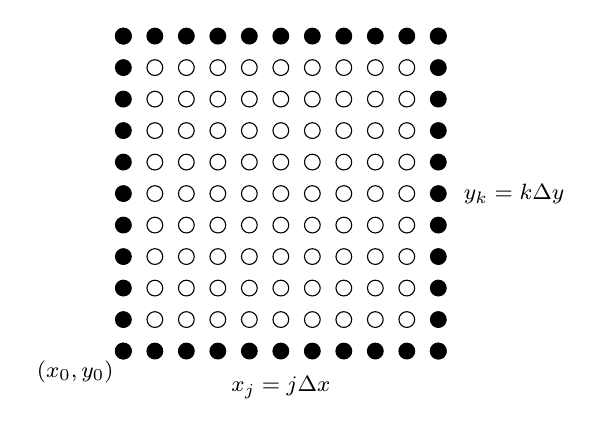
\begin{tikzpicture}

\foreach \x in {0,...,10}
{
\draw[fill=black] (0.4*\x,0) circle (0.1cm);
\draw[fill=black] (0.4*\x,4) circle (0.1cm);
}

\foreach \y in {0,...,10}
{
\draw[fill=black] (0,0.4*\y) circle (0.1cm);
\draw[fill=black] (4,0.4*\y) circle (0.1cm);
}

\foreach \x in {1,...,9}
\foreach \y in {1,...,9}
{
\draw[fill=white] (0.4*\x,0.4*\y) circle (0.1cm);
}
\fill (0,0) node[below left, font=\footnotesize] {$(x_0,y_0)$};
\fill (2,0) node[below, font=\footnotesize, yshift = -0.2cm] {$x_j=j\Delta x$};
\fill (4,2) node[right, font=\footnotesize, xshift = 0.2cm] {$y_k=k\Delta y$};
\end{tikzpicture}
\caption{Diagram of grid on which we approximate the potential $\phi$. White points
are interior points that change; black points are boundary points that remain constant.}
\end{figure}

\end{frame}

\begin{frame}{Discretisation of Laplace's equation}
Write $\phi(x,y)$ at $(x_j,y_k)$ as $\phi_{j,k}$.

Hence, Laplace's eqaution is discretised as
%
\be
\frac{\phi_{j+1,k}-2\phi_{j,k}+\phi_{j-1,k}}{\Delta x^2} + \frac{\phi_{j,k+1}-2\phi_{j,k}+\phi_{j,k-1}}{\Delta y^2}=0
\ee

For unique separation $\Delta = \Delta x = \Delta y$, $\phi_{j,k}$ is the average of the
surrounding points:
%
\be
\phi_{j,k}= \frac{1}{4}(\phi_{j+1,k}+\phi_{j-1,k}+\phi_{j,k+1}+\phi_{j,k-1})
\ee

\end{frame}

\section{Software}

\begin{frame}{Software Package}

Require software package capable of solving Laplace’s equation for different boundary
conditions. Developed \texttt{estatics} in C\texttt{++} that:
\begin{itemize}
\item accepts input of a coloured bitmap, colours represent regions of different constant potentials
\item converts to array of values depending on value assigned to each colour by the user
\item applies relaxation to array until all points have converged
\item outputs data files and plots of the resultant potential and electric field, and equipotential lines
\end{itemize}

\end{frame}

\begin{frame}{Flowchart}
\begin{figure}
\centerline{
\includegraphics[scale=0.7]{flowchart.pdf}
}
\end{figure}
\end{frame}

\subsection{Input}

\begin{frame}{Bitmap Boundary Conditions}

\begin{itemize}
\item Bitmap image files are used to input the boundary conditions.

\begin{figure}[H]
\centering
\includegraphics[width=0.4\textwidth]{bitmapA.pdf}
\caption{System A graphically represented as a BMP file.}
\end{figure}

\item Different colours represent different areas of constant potential.
\item The white pixels are areas of unsolved potential.

\end{itemize}

\end{frame}

\begin{frame}{Boolean Mask}

The locations of the boundary conditions and their potential are mapped on to two matrices.

\begin{itemize}
\item A matrix of potentials to be relaxed
\item A matrix of boolean values which stores the location of boundary values.
\end{itemize}

The boolean mask stores the location of:
\begin{itemize} 
\item boundary values as \lstinline|true|
\item other points to be iterated as \lstinline|false|.
\end{itemize}
When relaxation is applied to the matrix of potentials, values that are \lstinline|true|
are ignored, thus reducing computation time and preventing boundary decay.

\end{frame}

\subsection{Process}

\begin{frame}{Relaxation Methods}
Examined convergence of: 
\begin{itemize}
\item Jacobi iterative method,
\item Gauss-Seidel method,
\item successive over-relaxation.
\end{itemize}

Best was successive over-relaxation:
%
\be
\phi_{j,k,n+1}= (1-s)\phi_{j,k,n}+\frac{s}{4}(\phi_{j-1,k,n+1}+\phi_{j+1,k,n}+\phi_{j,k-1,n+1}+\phi_{j,k+1,n})
\ee
%
where $1<s<2$ is the \emph{relaxation parameter}.

\end{frame}

\begin{frame}{Checkerboard (Red-Black) Updating}

Denote $\phi_{j,k}$ as \emph{odd} if $j+k$ is odd, and even otherwise. Then:

\begin{itemize}
\item iterate through the grid
 \begin{itemize}
 \item update $\phi$ at each odd point (only depends on even points)
 \end{itemize}
\item re-iterate through grid
 \begin{itemize}
 \item update all even points using $\phi$ at newly updated odd points
 \end{itemize}
\end{itemize}

This is \emph{Checkerboard (Red-Black) Updating}
\begin{itemize}
\item separates system of $N$ linear equations into two coupled systems of
$\frac{N}{2}$ linear equations.
\item can have successive over-relaxation and parallel processing added
\end{itemize}

\end{frame}

\begin{frame}{Checkerboard (Red-Black) Updating cont.}
\begin{figure}[h!]
\begin{center}
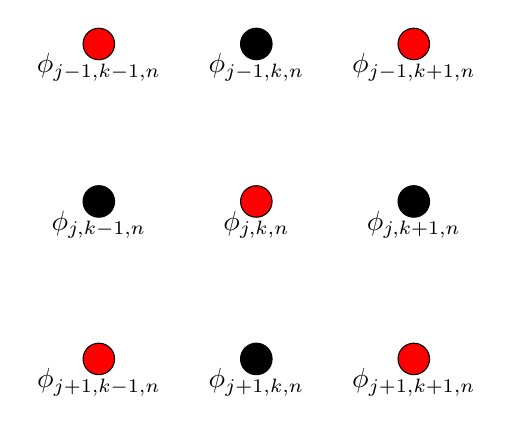
\begin{tikzpicture}
\draw[fill=red] (0,0) circle (0.2cm) node[below] {$\phi_{j+1,k-1,n}$};
\draw[fill=black] (2,0) circle (0.2cm) node[below] {$\phi_{j+1,k,n}$};
\draw[fill=red] (4,0) circle (0.2cm) node[below] {$\phi_{j+1,k+1,n}$};
\draw[fill=black] (0,2) circle (0.2cm) node[below] {$\phi_{j,k-1,n}$};
\draw[fill=red] (2,2) circle (0.2cm) node[below] {$\phi_{j,k,n}$};
\draw[fill=black] (4,2) circle (0.2cm) node[below] {$\phi_{j,k+1,n}$};
\draw[fill=red] (0,4) circle (0.2cm) node[below] {$\phi_{j-1,k-1,n}$};
\draw[fill=black] (2,4) circle (0.2cm) node[below] {$\phi_{j-1,k,n}$};
\draw[fill=red] (4,4) circle (0.2cm) node[below] {$\phi_{j-1,k+1,n}$};
\end{tikzpicture}
\end{center}
\caption{An illustration of checkerboard updating. The black points are updated first,
and then red points are calculated from the newly updated black points.}
\end{figure}

\end{frame}

\begin{frame}{Checkerboard (Red-Black) Updating cont.}
\begin{figure}[h!]
\begin{center}
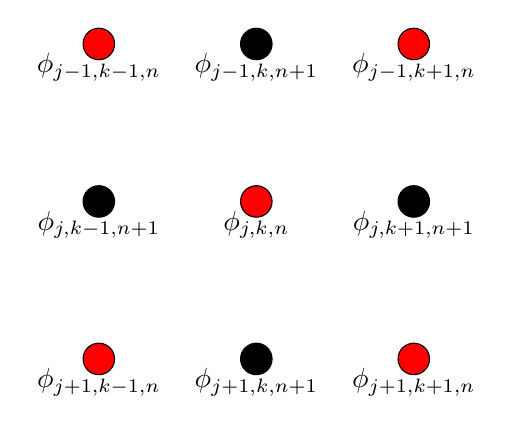
\begin{tikzpicture}
\draw[fill=red] (0,0) circle (0.2cm) node[below] {$\phi_{j+1,k-1,n}$};
\draw[fill=black] (2,0) circle (0.2cm) node[below] {$\phi_{j+1,k,n+1}$};
\draw[fill=red] (4,0) circle (0.2cm) node[below] {$\phi_{j+1,k+1,n}$};
\draw[fill=black] (0,2) circle (0.2cm) node[below] {$\phi_{j,k-1,n+1}$};
\draw[fill=red] (2,2) circle (0.2cm) node[below] {$\phi_{j,k,n}$};
\draw[fill=black] (4,2) circle (0.2cm) node[below] {$\phi_{j,k+1,n+1}$};
\draw[fill=red] (0,4) circle (0.2cm) node[below] {$\phi_{j-1,k-1,n}$};
\draw[fill=black] (2,4) circle (0.2cm) node[below] {$\phi_{j-1,k,n+1}$};
\draw[fill=red] (4,4) circle (0.2cm) node[below] {$\phi_{j-1,k+1,n}$};
\end{tikzpicture}
\end{center}
\caption{An illustration of checkerboard updating. The black points are updated first,
and then red points are calculated from the newly updated black points.}
\end{figure}

\end{frame}

\begin{frame}{Checkerboard (Red-Black) Updating cont.}
\begin{figure}[h!]
\begin{center}
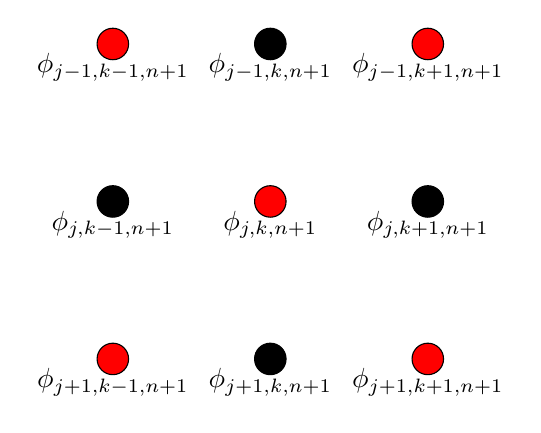
\begin{tikzpicture}
\draw[fill=red] (0,0) circle (0.2cm) node[below] {$\phi_{j+1,k-1,n+1}$};
\draw[fill=black] (2,0) circle (0.2cm) node[below] {$\phi_{j+1,k,n+1}$};
\draw[fill=red] (4,0) circle (0.2cm) node[below] {$\phi_{j+1,k+1,n+1}$};
\draw[fill=black] (0,2) circle (0.2cm) node[below] {$\phi_{j,k-1,n+1}$};
\draw[fill=red] (2,2) circle (0.2cm) node[below] {$\phi_{j,k,n+1}$};
\draw[fill=black] (4,2) circle (0.2cm) node[below] {$\phi_{j,k+1,n+1}$};
\draw[fill=red] (0,4) circle (0.2cm) node[below] {$\phi_{j-1,k-1,n+1}$};
\draw[fill=black] (2,4) circle (0.2cm) node[below] {$\phi_{j-1,k,n+1}$};
\draw[fill=red] (4,4) circle (0.2cm) node[below] {$\phi_{j-1,k+1,n+1}$};
\end{tikzpicture}
\end{center}
\caption{An illustration of checkerboard updating. The black points are updated first,
and then red points are calculated from the newly updated black points.}
\end{figure}

\end{frame}

\begin{frame}{Parallel Processing}

\begin{figure}
\begin{center}
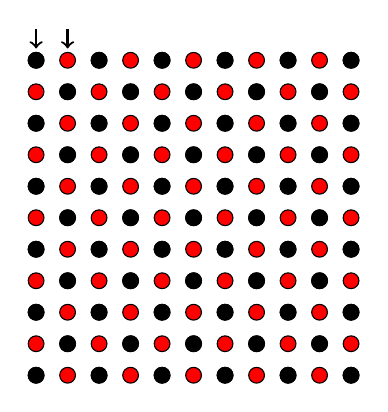
\begin{tikzpicture}
\foreach \x in {0,...,10}
{
 \foreach \y in {0,...,10}
 {
  \draw[fill=red] (0.4*\x,0.4*\y) circle (0.1cm);
 }
}

\foreach \x in {0,...,5}
{
 \foreach \y in {0,...,5}
 {
  \draw[fill=black] (0.8*\x,0.8*\y) circle (0.1cm);
 }
}

\foreach \x in {1,3,5,7,9}
{
 \foreach \y in {1,3,5,7,9}
 {
  \draw[fill=black] (0.4*\x,0.4*\y) circle (0.1cm);
 }
}

\draw[thick,->] (0,4.4) -- (0,4.15);
\draw[thick,->] (0.4,4.4) -- (0.4,4.15);

\end{tikzpicture}
\end{center}
\caption{An illustration of parallel processing. The black points in each and every
column are updated first, and then the red points in each and every column are
calculated from the newly updated black points.}
\end{figure}

\end{frame}

\begin{frame}{Parallel Processing cont.}

\begin{figure}
\begin{center}
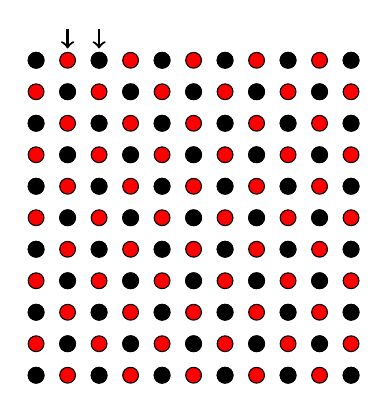
\begin{tikzpicture}
\foreach \x in {0,...,10}
{
 \foreach \y in {0,...,10}
 {
  \draw[fill=red] (0.4*\x,0.4*\y) circle (0.1cm);
 }
}

\foreach \x in {0,...,5}
{
 \foreach \y in {0,...,5}
 {
  \draw[fill=black] (0.8*\x,0.8*\y) circle (0.1cm);
 }
}

\foreach \x in {1,3,5,7,9}
{
 \foreach \y in {1,3,5,7,9}
 {
  \draw[fill=black] (0.4*\x,0.4*\y) circle (0.1cm);
 }
}

\draw[thick,->](0.4,4.4) -- (0.4,4.15);
\draw[thick,->] (0.8,4.4) -- (0.8,4.15);

\end{tikzpicture}
\end{center}
\caption{An illustration of parallel processing. The black points in each and every
column are updated first, and then the red points in each and every column are
calculated from the newly updated black points.}
\end{figure}

\end{frame}

\begin{frame}{Parallel Processing cont.}

\begin{figure}
\begin{center}
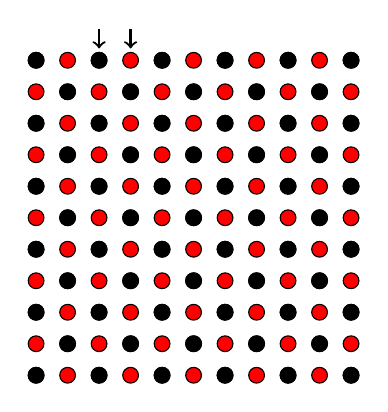
\begin{tikzpicture}
\foreach \x in {0,...,10}
{
 \foreach \y in {0,...,10}
 {
  \draw[fill=red] (0.4*\x,0.4*\y) circle (0.1cm);
 }
}

\foreach \x in {0,...,5}
{
 \foreach \y in {0,...,5}
 {
  \draw[fill=black] (0.8*\x,0.8*\y) circle (0.1cm);
 }
}

\foreach \x in {1,3,5,7,9}
{
 \foreach \y in {1,3,5,7,9}
 {
  \draw[fill=black] (0.4*\x,0.4*\y) circle (0.1cm);
 }
}

\draw[thick,->] (0.8,4.4) -- (0.8,4.15);
\draw[thick,->] (1.2,4.4) -- (1.2,4.15);

\end{tikzpicture}
\end{center}
\caption{An illustration of parallel processing. The black points in each and every
column are updated first, and then the red points in each and every column are
calculated from the newly updated black points.}
\end{figure}

\end{frame}

\begin{frame}{Convergence Limit}

The relaxation is terminated when every point is deemed to converge:
\begin{itemize}
\item Absolute convergence of each point is the difference between the potential of a
      point over successive iterations.
\item The system is iterated over until the absolute convergence of each point reduces below a desired value.
\item Converged point are treated as boundaries in the boolean mask and ignored during a pass over the grid.
\end{itemize}

\end{frame}

\begin{frame}{Convergence Lock}

Converged points are 'locked' and treated like a boundary condition to reduce
calculations per iteration.

\begin{figure}
 \centering
 \centerline{\includegraphics[width=0.5\textwidth]{lockvnolock.pdf}}
 \caption{The same system is solved with the lock on (red line) and the lock off (green line).}
\end{figure}

\begin{itemize}
\item The lock needs to be conditioned to not lock points too early.
\end{itemize}

\end{frame}

\begin{frame}{Convergence Locking Cont.}
\begin{figure}
\centering
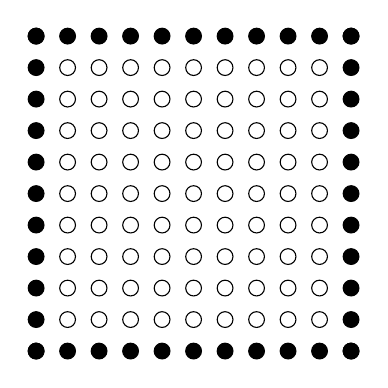
\begin{tikzpicture}

\foreach \x in {0,...,10}
{
\draw[fill=black] (0.4*\x,0) circle (0.1cm);
\draw[fill=black] (0.4*\x,4) circle (0.1cm);
}

\foreach \y in {0,...,10}
{
\draw[fill=black] (0,0.4*\y) circle (0.1cm);
\draw[fill=black] (4,0.4*\y) circle (0.1cm);
}

\foreach \x in {1,...,9}
{
 \foreach \y in {1,...,9}
 {
 \draw[fill=white] (0.4*\x,0.4*\y) circle (0.1cm);
 }
}

\end{tikzpicture}
\caption{Illustration of convergence locking. As relaxation is applied more points converge and are locked.}
\end{figure}

\end{frame}

\begin{frame}{Convergence Locking Cont.}
\begin{figure}
\centering
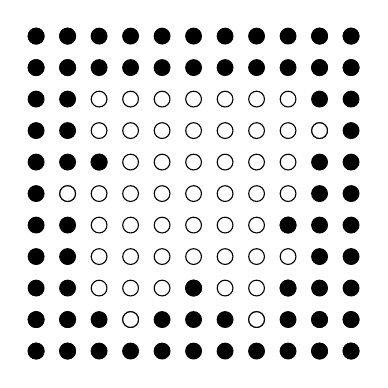
\begin{tikzpicture}

\foreach \x in {0,...,10}
{
\draw[fill=black] (0.4*\x,0) circle (0.1cm);
\draw[fill=black] (0.4*\x,0.4) circle (0.1cm);
\draw[fill=black] (0.4*\x,3.6) circle (0.1cm);
\draw[fill=black] (0.4*\x,4) circle (0.1cm);
}

\foreach \y in {0,...,10}
{
\draw[fill=black] (0,0.4*\y) circle (0.1cm);
\draw[fill=black] (0.4,0.4*\y) circle (0.1cm);
\draw[fill=black] (3.6,0.4*\y) circle (0.1cm);
\draw[fill=black] (4,0.4*\y) circle (0.1cm);
}

\foreach \x in {2,...,8}
{
 \foreach \y in {2,...,8}
 {
 \draw[fill=white] (0.4*\x,0.4*\y) circle (0.1cm);
 }
}

%add random (un)converged points, increment of 0.4
\draw[fill=black] (3.2,1.6) circle (0.1cm);
\draw[fill=black] (0.8,2.4) circle (0.1cm);
\draw[fill=black] (2,0.8) circle (0.1cm);
\draw[fill=black] (3.2,0.8) circle (0.1cm);

\draw[fill=white] (1.2,0.4) circle (0.1cm);
\draw[fill=white] (2.8,0.4) circle (0.1cm);
\draw[fill=white] (0.4,2) circle (0.1cm);
\draw[fill=white] (3.6,2.8) circle (0.1cm);

\end{tikzpicture}
\caption{Illustration of convergence locking. As relaxation is applied more points converge and are locked.}
\end{figure}

\end{frame}

\begin{frame}{Convergence Locking Cont.}
\begin{figure}
\centering
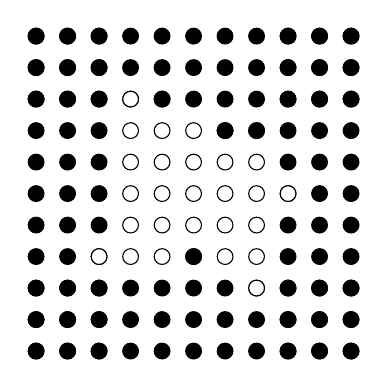
\begin{tikzpicture}

\foreach \x in {0,...,10}
{
\draw[fill=black] (0.4*\x,0) circle (0.1cm);
\draw[fill=black] (0.4*\x,0.4) circle (0.1cm);
\draw[fill=black] (0.4*\x,0.8) circle (0.1cm);
\draw[fill=black] (0.4*\x,3.2) circle (0.1cm);
\draw[fill=black] (0.4*\x,3.6) circle (0.1cm);
\draw[fill=black] (0.4*\x,4) circle (0.1cm);
}

\foreach \y in {0,...,10}
{
\draw[fill=black] (0,0.4*\y) circle (0.1cm);
\draw[fill=black] (0.4,0.4*\y) circle (0.1cm);
\draw[fill=black] (0.8,0.4*\y) circle (0.1cm);
\draw[fill=black] (3.2,0.4*\y) circle (0.1cm);
\draw[fill=black] (3.6,0.4*\y) circle (0.1cm);
\draw[fill=black] (4,0.4*\y) circle (0.1cm);
}

\foreach \x in {3,...,7}
{
 \foreach \y in {3,...,7}
 {
 \draw[fill=white] (0.4*\x,0.4*\y) circle (0.1cm);
 }
}

%add random (un)converged points, increment of 0.4
\draw[fill=black] (2.4,2.8) circle (0.1cm);
\draw[fill=black] (1.6,3.2) circle (0.1cm);
\draw[fill=black] (2,1.2) circle (0.1cm);
\draw[fill=black] (2.8,2.8) circle (0.1cm);

\draw[fill=white] (2.8,0.8) circle (0.1cm);
\draw[fill=white] (1.2,3.2) circle (0.1cm);
\draw[fill=white] (0.8,1.2) circle (0.1cm);
\draw[fill=white] (3.2,2) circle (0.1cm);

\end{tikzpicture}
\caption{Illustration of convergence locking. As relaxation is applied more points converge and are locked.}
\end{figure}

\end{frame}

\begin{frame}{Convergence Locking Cont.}
\begin{figure}
\centering
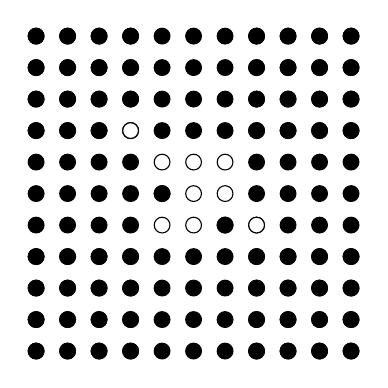
\begin{tikzpicture}

\foreach \x in {0,...,10}
{
\draw[fill=black] (0.4*\x,0) circle (0.1cm);
\draw[fill=black] (0.4*\x,0.4) circle (0.1cm);
\draw[fill=black] (0.4*\x,0.8) circle (0.1cm);
\draw[fill=black] (0.4*\x,1.2) circle (0.1cm);
\draw[fill=black] (0.4*\x,2.8) circle (0.1cm);
\draw[fill=black] (0.4*\x,3.2) circle (0.1cm);
\draw[fill=black] (0.4*\x,3.6) circle (0.1cm);
\draw[fill=black] (0.4*\x,4) circle (0.1cm);
}

\foreach \y in {0,...,10}
{
\draw[fill=black] (0,0.4*\y) circle (0.1cm);
\draw[fill=black] (0.4,0.4*\y) circle (0.1cm);
\draw[fill=black] (0.8,0.4*\y) circle (0.1cm);
\draw[fill=black] (1.2,0.4*\y) circle (0.1cm);
\draw[fill=black] (2.8,0.4*\y) circle (0.1cm);
\draw[fill=black] (3.2,0.4*\y) circle (0.1cm);
\draw[fill=black] (3.6,0.4*\y) circle (0.1cm);
\draw[fill=black] (4,0.4*\y) circle (0.1cm);
}

\foreach \x in {4,...,6}
{
 \foreach \y in {4,...,6}
 {
 \draw[fill=white] (0.4*\x,0.4*\y) circle (0.1cm);
 }
}

%add random (un)converged points, increment of 0.4
\draw[fill=black] (2.4,1.6) circle (0.1cm);
\draw[fill=black] (1.6,2) circle (0.1cm);

\draw[fill=white] (2.8,1.6) circle (0.1cm);
\draw[fill=white] (1.2,2.8) circle (0.1cm);

\end{tikzpicture}
\caption{Illustration of convergence locking. As relaxation is applied more points converge and are locked.}
\end{figure}

\end{frame}

\begin{frame}{Convergence Locking Cont.}
\begin{figure}
\centering
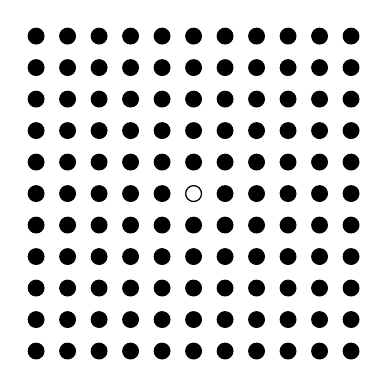
\begin{tikzpicture}

\foreach \x in {0,...,10}
{
 \foreach \y in {0,...,10}
 {
  \draw[fill=black] (0.4*\x,0.4*\y) circle (0.1cm);
 }
}

\draw[fill=white] (2,2) circle (0.1cm);

\end{tikzpicture}
\caption{Illustration of convergence locking. As relaxation is applied more points converge and are locked.}
\end{figure}

\end{frame}

\begin{frame}{Convergence Locking Cont.}
\begin{figure}
\centering
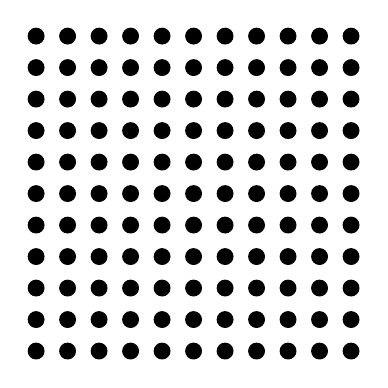
\begin{tikzpicture}

\foreach \x in {0,...,10}
{
 \foreach \y in {0,...,10}
 {
  \draw[fill=black] (0.4*\x,0.4*\y) circle (0.1cm);
 }
}
\end{tikzpicture}
\caption{Illustration of convergence locking. As relaxation is applied more points converge and are locked.}
\end{figure}

\end{frame}

\section{Results}

\begin{frame}{Results}
\end{frame}

\section{Analysis}
\begin{frame}{Analysis}
\end{frame}

\section{Conclusion}

\begin{frame}{Conclusion}
Further Work:
\begin{itemize}
\item Other elliptic PDEs e.g. Poisson's equation
\item Boundary conditions that vary with position
\end{itemize}

Alternative methods:
\begin{itemize}
\item Multigrid methods
\item Fast Fourier Transform
\item Nine-point stenciling
\end{itemize}

\end{frame}

\begin{frame}
\titlepage
\end{frame}

\end{document} %end of document
